\documentclass[a4paper,12pt]{article}
\usepackage[utf8]{inputenc}
\usepackage[T1]{fontenc}
\usepackage[francais]{babel}
\usepackage{graphicx}
\usepackage[left=2cm,right=2cm,top=2cm,bottom=2cm]{geometry}
\pagestyle{plain}

\title{BE de Cyber Physiques}
\author{Grégoire Martini \& Félix Schaller }
\date{23 Mai 2016}

\begin{document}
\maketitle

\bigskip
\bigskip
\bigskip
\tableofcontents
\newpage


\section{TP1 : Modèle continu du pendule simple}
\subparagraph{Modèle}

On cherche à modéliser le comportement d'un pendule simple. Le système d'équation physique est le suivant :

\begin{center}
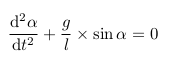
\includegraphics[width=4cm]{./img/tp1_eq.png}
\end{center}


Pour résoudre cette équation avec Simulink nous utilisons d'abord deux intégrateurs différents. Nous avons aussi fait apparaître explicitement les conditions initiales pour faciliter les simulations.

\begin{center}
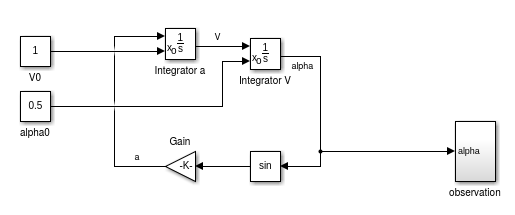
\includegraphics[width=13cm]{./img/tp1.png}
\end{center}

\subparagraph{Simulation}

Pour faciliter nos observations, nous avons créé un sous-système \textit{observation} qui affiche l'angle pris le pendule et la position de l'extrémité de la tige sur un graphe XY. Nous reprendrons ce sous-système pour chaque simulation.

\begin{center}
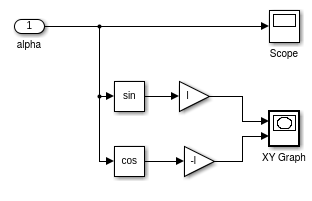
\includegraphics[height=5cm]{./img/obs.png}
\end{center}

\clearpage

Voici les résultats de notre simulation avec les paramètres suivants:
\
\begin{itemize}
\item[l = 0.072 m]
\item[V0 = 1 rad/s]
\item[alpha0 = 0.5 rad]
\end{itemize}

\begin{center}
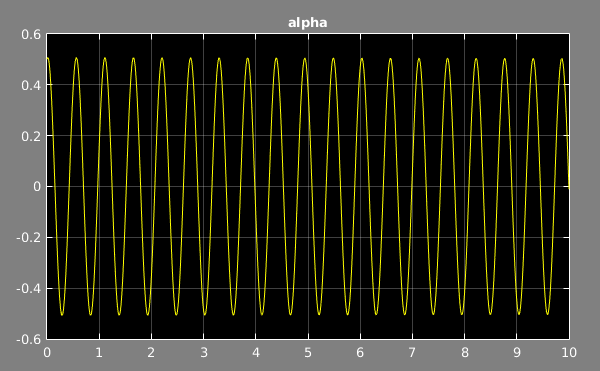
\includegraphics[width=10cm]{./img/tp1_alpha.png}
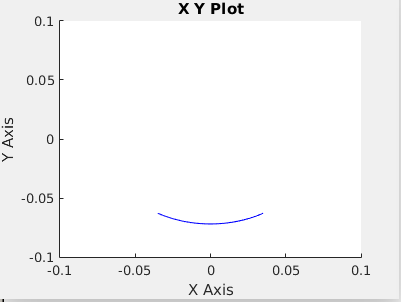
\includegraphics[width=6cm]{./img/tp1_xy.png}
\end{center}

\subparagraph{Analyse}

Une position d'équilibre du pendule est à alpha = 0.
Le système proposé ici ne prend pas en compte l'amortissement dû aux frottements, le point d'équilibre n'est donc pas asymptotiquement stable. Le système ayant été lancé avec une vitesse initiale et un angle non nuls, il oscille indéfiniment autour de cette position.


\clearpage
\section{TP2 : Modèle continu structuré}
\subsection{Pendule simple}

Il s'agit du même système que le TP précédent. Le but ici était de résoudre le système avec un seul intégrateur comme le modèle Simulink suivant.

\begin{center}
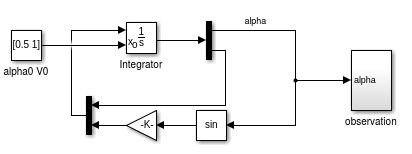
\includegraphics[width=10cm]{./img/tp2_ps.png}
\end{center}

Nous avons donc utiliser un vecteur $x = <\alpha, \frac{d\alpha}{dt}> $ pour résoudre le problème.\\

Nous avons aussi vérifié que obtenions les mêmes résultats de simulation à partir des mêmes conditions initiales.

\subsection{Pendule inversé avec contrôleur par retour d'état}
\subparagraph{Modèle}

On cherche à modéliser le comportement d'un pendule inversé avec contrôle par retour d'état. Le système d'équation physique est le suivant :

\begin{center}
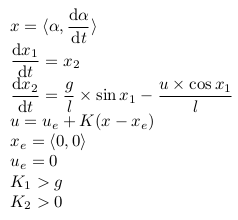
\includegraphics[width=6cm]{./img/tp2_eq.png}
\end{center}

Pour résoudre le système ci-dessus, nous avons utilisons les mêmes techniques que précédemment. Nous avons créé un sous-système pour le calcul de u et non avons ajouté une perturbation à la vitesse angulaire sous la forme d'un signal rectangulaire.

\begin{center}
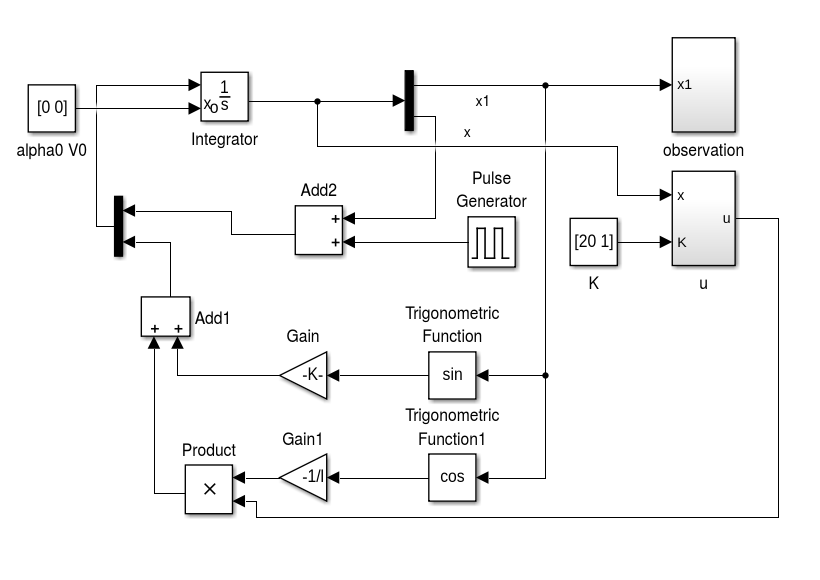
\includegraphics[width=14cm]{./img/tp2_pi.png}
\end{center}

\subparagraph{Simulation}

Nous avons remplacé nos conditions initiales pour nous placer au point d'équilibre alpha = 0 du pendule inversé avec une vitesse initiale nulle et la longueur de la tige l = 0.072 m est restée identique.
Nous avons utilisé une perturbation d'amplitude 1 rad/s pendant 500 ms à la deuxième seconde de chaque simulation. 
Pour n'avoir qu'une perturbation sur les dix secondes de la simulation nous avons choisi une période de dix secondes avec un rapport cyclique de 5\%.

\begin{center}
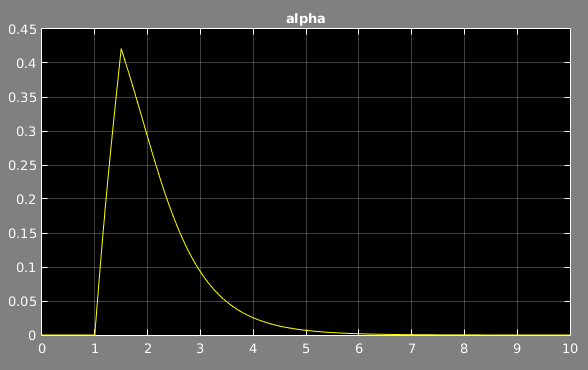
\includegraphics[width=8cm]{./img/tp2_11_1.png}
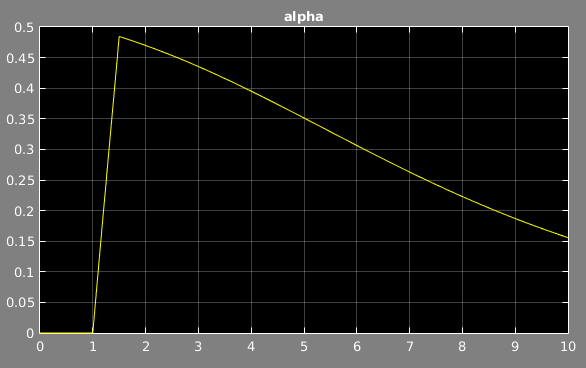
\includegraphics[width=8cm]{./img/tp2_11_6.png}\\
\textit{K1 = 11,  K2 = 1 } \hspace{5cm} \textit{K1 = 11,  K2 = 6 }
\bigskip

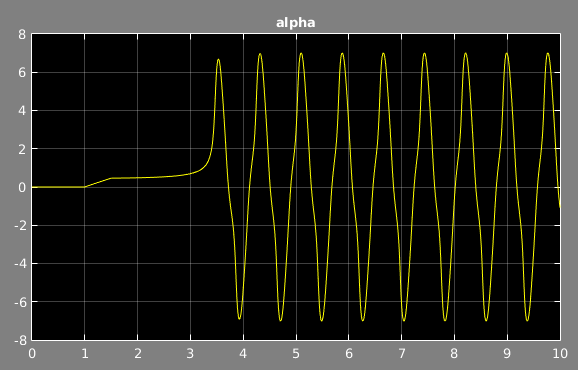
\includegraphics[width=8cm]{./img/tp2_10,5_1.png}\\
\textit{K1 = 10.5,  K2 = 1 }
\end{center}

\subparagraph{Analyse}

Pour les deux premières simulations on constate qu'un coefficient de valeur 11 sur le contrôleur proportionnel permet un retour à la position d'équilibre alors que sur la troisième simulation une valeur de 10.5 ne le permet pas.
En effet, plus la valeur du coefficient proportionnel est grand plus le retour à la valeur de consigne est rapide.\\
Les deux premières simulations permettent d'étudier l'influence du coefficient dérivateur, celui-ci ralenti le temps de réponse du contrôleur.


\clearpage
\section{TP4 : Modèle continu et discret du robot Lego}
\subsection{Modèle continu}
\subparagraph{Modèle}

\begin{center}
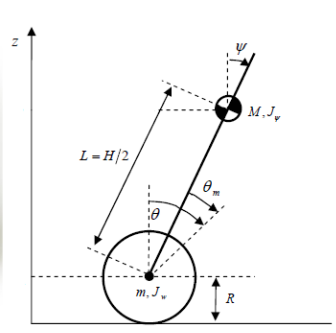
\includegraphics[height=6cm]{./img/robot.png}
\end{center}

\subparagraph{Simulation}
\subparagraph{Analyse}

var k1, k2 k3 k4 trouvé par calcul
analyse estimateur

CODE A FAIRE

\subsection{Modèle discret}
\subparagraph{Modèle}
\subparagraph{Simulation}
\subparagraph{Analyse}

dito


\clearpage
\section{TP5-6 : Application embarquée sur le robot Lego}
\subparagraph{Modèle}

Pour reconstruire les données nécessaires au contrôle du robot nous utilisons une méthode estimateur. Pour intégrer ou dériver une valeur nous utilisons la formule du taux d'accroissement sachant que le relevé des mesures est effectué à intervalle de temps régulier dt.

\begin{center}
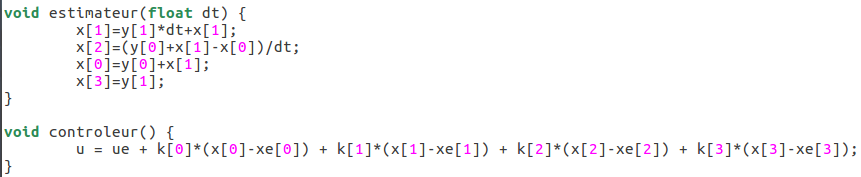
\includegraphics[width=17cm]{./img/tp5_c.png}
\end{center}

\subparagraph{Exécution}

Lors de l'exécution sur le robot segway, nous n'avons pas testé nos valeurs pour le K car nous savions qu'elle n'étaient pas cohérentes. En effet, lors de son calcul, nous étions partis des valeurs propres de la matrice A (cf TP4). Nous avons donc utilisé les valeurs données par notre enseignant de TP pour faire rouler notre robot.

Nous avons pu constater lors de ces tests que si nous ne laissions pas suffisamment de temps pour l'initialisation de gyroscope alors le robot se mettait à avancer ou tombait.


\end{document}          

